\documentclass{article}
\usepackage{CJK}
\usepackage{amsmath,amssymb}
\usepackage{geometry,graphicx}
\geometry{bottom = 3cm, left = 3cm, right = 3cm, top = 3cm}
\title{数值分析说明文档}
\author{张奇 PB19000093}
\begin{document}
\begin{CJK}{UTF8}{gbsn}
    	\maketitle
    \section{实验内容}
    	\paragraph{实验一}本次实验实现Lagrange积分:均匀节点和Chebysheff节点选取以计算数值积分。
    	\begin{itemize}
    		\item $\{f(x) = \dfrac{1}{25x^2+1}\}$
    		\item $\{x_i^1 = 1 - 2\dfrac{i}{N}\},\{x_i^2 = \cos(\pi\frac{i+1}{N+2})\}  N = 5,10,15,\cdots, 50. $
    		\item 比较误差$|\int_{-1}^1 f - \int_{-1}^1 p_{uniform}|,  |\int_{-1}^1 f - \int_{-1}^1 p_{Chebysheff}|.$并且输出结果。
    	\end{itemize}。
    	\paragraph{实验二}计算估计积分$\int_0^\infty \cos^2 x e^{-x} dx$的截断误差 $\int_c^\infty \cos^2 x e^{-x} dx < 10^{-3}$的条件。
    \section{算法实现}
		\paragraph{实验一}
			我的基本思路是:将按照固定节点的Lagrange基函数的积分方法计算出来,这需要将Lagrange基函数展开,可以考虑用一个数据结构来模拟这个过程,最后在逐个指数计算结果,最后用Lagrange基函数的积分对上函数的直,得到解。最后输出
		\paragraph{实验二}
			我的基本思路是:将之积分计算是可以计算出来的,然后递归查找就可以了,
			\begin{align}
				\int_c^\infty \cos^2 x e^{-x} dx & = \int_c^\infty \frac{1 +  \cos 2x}{2} e^{-x} \\
				 & = \frac{e^{-x}}{2} + \frac{\mbox{Re}(\int_c^\infty e^{(2i-1)x} )}{2} \\
				 & = (1+\frac{\cos 2c - 2 \sin 2c}{5}) \frac{e^{-c}}{2}
			\end{align}
    	\section{编译环境}
    	\begin{itemize}
    		\item 编译器:g++ (Ubuntu 9.4.0-1ubuntu1~20.04.1) 9.4.0.
    		\item 编译命令:./run  code6( 实验一) ./run  code6hw  (实验二)
    	\end{itemize}
    \section{结果总结}
    \begin{figure}[hbpt]
    	\centering
    	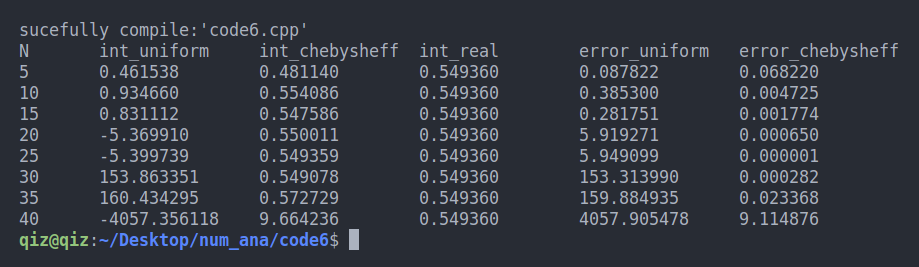
\includegraphics[width=0.6\linewidth]{code6.png}
    	\caption{\textbf{实验一:}误差估计}
    	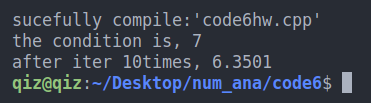
\includegraphics[width=0.6\linewidth]{code6hw.png}
    	\caption{\textbf{实验二:}结果分析}
    \end{figure}
		
    \paragraph{分析}
\end{CJK}
\end{document}